\chapter{Resugaring Evaluation Sequences}\label{chap:resugar-eval}

% Greek αβγδε

In this chapter, we tackle the challenge of combining syntactic sugar with
semantics. Given a set of desugaring rules written in the style of the
last chapter, we show how to resugar \emph{program execution}:
to automatically convert an
evaluation sequence in the core language into a representative
evaluation sequence in the surface syntax. Each step in the surface
language emulates one or more steps
in the core language. The computed steps hide the desugaring, thus
maintaining the abstraction provided by the surface language.

The chief challenge is to
remain faithful to the original semantics---we can't change the meaning of
a program!---and to ensure that the internals of the code introduced by
the syntactic sugar does not leak into the output. Our chief mechanisms
for achieving this are to (a) perform static checks on the desugaring
rules to ensure they fall into the subset we can handle, and (b)
rewrite the reduction relation with instrumentation to track the origin of
terms. We implement these ideas in a tool called {\Resugarer}, and
formally verify key properties of our approach, given simplifying
assumptions, in the Coq proof assistant.

This chapter comes from work published in PLDI 2014 and ICFP 2015
under the titles of \emph{Resugaring: Lifting Evaluation Sequences
  through Syntactic Sugar} and \emph{Hygienic Resugaring of
  Compositional Desugaring} (both co-authored with Shriram
Krishnamurthi)~\cite{pombrio-resugar,pombrio-resugar-hygienic}.


\section{Our Approach}

We aim to compute sensible evaluation sequences in a surface language,
while remaining faithful to the core language's semantics.  One approach
would be to attempt to construct a lifted (to the surface language)
reduction-relation directly. It is unclear, however, how to do this
without making deep assumptions about the core language evaluator
(for instance, assuming that it is defined as a term-rewriting system that can be composed
with desugaring).

Our approach instead makes minimal assumptions about the
evaluator, treating it as a black-box (since it is often a complex
program that we may not be able to modify).
We assume only that we have access to a \emph{stepper} that
provides a sequence of evaluation steps (augmented with some
meta information) in the \emph{core} language. In 
\cref{sec:reval-lang} we show how to obtain such a stepper from a generic,
black-box
evaluator with a strategy that can be implemented by pre-processing
the program before evaluation.

Our high-level approach is to follow the evaluation steps in the core
language, find surface-level representations of some of the core
terms, and emit them. Not every core-level term will have a
surface-level representation; these steps will be skipped in the
output. The evaluation sequence shown, then, is the sequence of
surface-level representations of the core terms that were not
skipped. Central to this approach are three properties:

\begin{description}
\item[Emulation] Each term in the generated surface evaluation
  sequence desugars into the core term which it is meant to represent
  (up to term isomorphism).
\item[Abstraction] Code introduced by desugaring is never revealed in the
  surface evaluation sequence, and code originating from the original
  input program is never hidden by resugaring.
\item[Coverage] Resugaring is attempted on every core step, and as few
  core steps are skipped as possible.
%\item[Hygiene] Both desugaring and resugaring preserve
%  $\alpha$-equivalence on terms.
\end{description}

\section{Informal Solution Overview}
\label{sec:reval-exposition}

We first present the techniques used by our solution, and some subtleties,
informally. We choose a familiar desugaring example: the rewriting
of \Code{Or}, as used in languages like Lisp and Scheme. We assume
the surface language has \Code{Or} as a construct, while the core does
not. We present our examples using a traditional infix concrete syntax.

% Unexpansion
\subsection{Finding Surface Representations Preserving Emulation}

We start by defining a simple, binary version of \Code{Or} (that
let-binds its first argument in case it has side-effects):\marginpar{%
We present these examples using the actual syntax of {\Resugarer},
which uses {\normalfont \Code{x}} instead of $\alpha$ for a pattern variable, and
represents variables as strings.}
\begin{Codes}
Or(x, y) -> Let([Binding("t", x)],
                If(Id("t"), Id("t"), y)));
\end{Codes}
In this section we focus on abstract syntax and ignore
the mapping to it from concrete syntax.

Consider the surface term \Code{not(true) OR not(false)}. After
desugaring, this would evaluate as follows in the core language
(assuming a typical call-by-value evaluator):
\begin{Codes}
    let t = not(true) in
      if t then t else not(false)
\CoreStep let t = false in
      if t then t else not(false)
\CoreStep if false then false else not(false)
\CoreStep not(false)
\CoreStep true
\end{Codes}
In the surface language, we would wish to see this as (using dashed
arrows to denote reconstructed steps):
\begin{Codes}
    not(true) OR not(false)
\SurfStep false OR not(false)
\SurfStep not(false)
\SurfStep true
\end{Codes}
The first two terms in the core evaluation sequence are precisely the
expansions of the first two steps in the (hypothetical) surface evaluation
sequence. This suggests
we can \emph{unexpand} core terms into surface terms by running rules ``in
reverse'': matching against the \Sc{rhs} and substituting into the
corresponding \Sc{lhs}.
(To preserve Emulation, unexpansion must be an inverse of expansion: we
prove that this is so in \cref{sec:reval-inverses}.)
We will now show how the last two steps
may come about.

\subsection{Maintaining Abstraction}
\label{sec:reval-exposition-tagging}

When unexpanding, we should only unexpand code that
originated from a sugar. If the surface program itself is
\begin{Codes}
let t = not(true) in
  if t then t else not(false)
\end{Codes}
it should not unexpand into \Code{not(true) OR not(false)}:
this would be confusing and break the second clause of the Abstraction property.

We therefore augment each subterm in a core term
with a list of \emph{tags}, which indicate whether a term
originated in the original source or from sugar.%
\marginpar{Whereas the tags used in hygienic macro
  expansion~\cite{hygienic-macros} specify time steps,
  the tags in resugaring specify which sugar the
  code originated from.}
Unexpansion attempts to process terms marked as
originating from a desugaring rule; this
unexpansion will fail if the tagged term no longer has the form of
the rule's \Sc{rhs}. When this happens, we conclude that there is no
surface representation of the core term and skip the step.

To illustrate this, we revisit the same core evaluation sequence as
before. \newline %NEWLINE
``\Code{\{Head$_\texttt{Or}$:~\}}'' is a tag on the desugared expression that
indicates it originated from the \Code{Or} sugar, and ``\Code{\{Body:~\}}''
is a tag that indicates it originated from sugar (without saying
which, although in this case it came from \Code{Or}):
\begin{Codes}
    \{Head\(\sb{\texttt{Or}}\): let t = not(true) in
      \{Body: if t then t else not(false)\}\}
\CoreStep \{Head\(\sb{\texttt{Or}}\): let t = false in
      \{Body: if t then t else not(false)\}\}
\CoreStep \{Body: if false then false else not(false)\}
\CoreStep not(false)
\CoreStep true
\end{Codes}
The tags on the first two steps suggest that \Code{Or}'s
desugaring rule be applied in reverse. They can be unexpanded
because they match the \Sc{rhs} of \Code{Or}. The third step fails to
resugar because the \Code{if} is never unexpanded, and thus is a
leftover fragment of sugar. This step is therefore skipped, yielding no
surface step. The last two steps are not tagged and are
therefore included in the surface evaluation sequence as-is.

\subsection{Striving for Coverage}

Emulation and Abstraction guarantee an accurate
surface evaluation sequence, but they do not guarantee a useful one. For
instance, the following evaluation sequence is perfectly consistent with
these two properties:
\begin{Codes}
    not(true) OR not(false)
\SurfStep true
\end{Codes}
However, a stepper that only shows the final step is unhelpful. We therefore
propose a third property, Coverage, which states that steps
are not ``unnecessarily'' skipped. While Emulation and
Abstraction are formally proved in \cref{sec:reval-proofs}, we have not found a
complete formalization of Coverage, so we can only strive to attain it in
our systems and evaluate it in practice.\marginpar{%
A \emph{partial} formalization of coverage can be found in the second
paper this chapter is based on~\cite{pombrio-resugar-hygienic}.
}
Our examples
(\cref{sec:reval-pyret-example} and \cref{sec:reval-examples}) show
that we do indeed obtain detailed and useful surface evaluation sequences.

\subsection{Trading Abstraction for Coverage}
\label{sec:reval-trading}

Suppose the surface term \Code{A OR B OR C} parses to
\Code{Or(A, B, C)}. We therefore want to extend \Code{Or}
to handle more than two sub-terms.  We can do this by adding another
rule:
\begin{Codes}
Or([x, y]) ->
  Let([Binding("t", x)],
      If(Id("t"), Id("t"), y)));
Or([x, y, ys ...] ->
  Let([Binding("t", x)],
      If(Id("t"), Id("t"), Or([y, ys ...])));
\end{Codes}
We assume a prioritized semantics in which rules are tried in
order; the first rule whose \Sc{lhs} matches the invocation is
used. The ellipses denote zero or more repetitions
of the preceding pattern~\cite{macro-by-example}.

Consider the surface term \Code{(false OR false OR true)}. 
Given the revised definition of \Code{Or}, unexpansion would yield the
following lifted evaluation steps:
\begin{Codes}
    false OR false OR true
\SurfStep true
\end{Codes}
In particular, it correctly suppresses any presentation of the recursive
invocation of \Code{Or}
introduced by desugaring---precisely what Abstraction demands!
However, there are settings
(such as debugging or education) where the user might wish to see this
invocation, i.e., to obtain the surface evaluation sequence:
\begin{Codes}
    false OR false OR true
\SurfStep false OR true
\SurfStep true
\end{Codes}
Thus, we let sugar authors make part of a rule's \Sc{rhs}
visible by prefixing it with \Code{!}. Here, writing the second
\Code{Or} rule as:
\begin{Codes}
Let([Binding("t", x)],
    If(Id("t"), Id("t"), !Or([y, ys ...])))
\end{Codes}
yields the latter surface evaluation sequence.

This illustrates that there is a trade-off (which we make precise with
\cref{thm:reval-abstraction}) between Abstraction and Coverage.
Because the trade-off depends on
goals, we entrust it to the sugar author.  In the limit,
marking the entirety of each rule as transparent results in
an ordinary trace in the core, ignoring all sugar.

\subsection{Maintaining Hygiene}

The implementation discussed in this
chapter---{\Resugarer}---represents variables as strings and is not
hygienic. The next chapter, \cref{sec:rscope-eval-hygiene}, shows how
to fix this. Three changes must be made: (i) sugars must pass that
chapter's \emph{scope inference} algorithm; (ii) introduced variables
must (unsurprisingly) be given fresh names, and resugaring must allow
introduced variables to match against any name; and (iii) sugars must
not drop pattern variables. Given these changes,
\cref{sec:rscope-eval-hygiene} proves that both desugaring and
resugaring will be hygienic.

\section{{\Resugarer} at Work}
\label{sec:reval-pyret-example}

We demonstrate how the techniques just described come together to show
surface evaluation sequences in the presence of sugar. Consider the
following program, written in the language Pyret (\url{pyret.org}), 
that computes the length of a list:
\begin{Codes}
    fun len(x):
      cases(List) x:
        | empty() => 0
        | link(_, tail) => len(tail) + 1
      end
    end
    len([1, 2])
\end{Codes}
This seemingly innocuous program contains a lot of sugar. The \Code{cases}
expression desugars into an application of the matchee's \Code{\_match}
method on an object containing code for each branch; the function
declaration desugars into a let binding to a lambda; addition desugars
into an application of a \Code{\_plus} method; and the list \Code{[1, 2]}
desugars into a chain of list constructors. Here is the full desugaring
(i.e., the code that will actually be run):
\begin{Codes}
len = fun(x):
    temp17 :: List = x
    temp17.["_match"](
      \{"empty" : fun(): 0 end,
       "link" : fun(_, tail):
                len(tail).["_plus"](1) end\},
      fun(): raise("cases: no cases matched");)
    end
len(list.["link"](1, list.["link"](2, list.["empty"])))
\end{Codes}
This degree and nature of expansion is not unique to Pyret.
It is also found in languages like Scheme, due
to the small size of the core, and in semantics like
$\lambda_{JS}$~\cite{lambda-js},
due to both the size of the core and the enormous complexity
of the surface language.

Nevertheless, here is the surface evaluation (pretty-)printed by {\Resugarer} (where
\Code{<func>} denotes a resolved functional):
\begin{Codes}
\SurfStep <func>([1, 2])
\SurfStep cases(List) [1, 2]:
      | empty() => 0
      | link(_, tail) => len(tail) + 1
    end
\SurfStep <func>([2]) + 1
\SurfStep (cases(List) [2]:
      | empty() => 0
      | link(_, tail) => len(tail) + 1
    end) + 1
\SurfStep <func>([]) + 1 + 1
\SurfStep (cases(List) []:
      | empty() => 0
      | link(_, tail) => len(tail) + 1
    end) + 1 + 1
\SurfStep 0 + 1 + 1
\SurfStep 1 + 1
\SurfStep 2
\end{Codes}
This sequence hides all the complexity of the core language.


\section{The Transformation System}
\label{sec:reval-transformations}

We will present our system in three parts. First
(\cref{sec:reval-onerule}), we will describe how our transformation system
works, up to the level of performing a single \emph{transformation}:
either expanding or unexpanding a single (instance of a) sugar. Next
(\cref{sec:reval-manyrule}), we will describe how to use tags to fully
desugar and resugar terms, transforming not just a term but its subterms
as well. Finally (\cref{sec:reval-lifting}), we will show how to use the
transformation system to lift core evaluation sequences to surface
evaluation sequences.

\subsection{Performing a Single Transformation}
\label{sec:reval-onerule}

We begin by describing the form and application of our transformation
rules.

\subsubsection{Patterns}

Since rules are applied both forward and in reverse, we represent their
\Sc{lhs}s and \Sc{rhs}s uniformly as \emph{patterns}. We give a
broader definition of patterns here than in \cref{sec:formal-term}:
here we allow patterns to contain lists, ellipses, and (for the
purposes of resugaring) tags.

\begin{Table}
pattern $p$ &$::=$& $\PVarA$ & pattern variable \\
  &$|$& $\Node{C}{p_1 ... p_n}$ & \Sc{ast} node \\
  &$|$& $[p_1 \dd p_n]$ & list of length $n$ \\
  &$|$& $[p_1 \dd p_n\,\Ell{p}]$ & list of length $\geq n$ (ellipses) \\
  &$|$& $\Value$ & primitive value \\
  &$|$& $\VarX$  & variable \\
  &$|$& $\Tag{o}{p}$ & origin tag \\ \\
term $e$ &$::=$& $p$ & pattern w/o pattern variables or ellipses \\ \\
origin tag $o$ &$::=$&
        $\MacHead{i}{e}$& marks topmost rule production \\
  &$|$& $\MacBody{\textit{bool}}$   & marks each rule production
\end{Table}

Variables are denoted by a lowercase
identifier (we omit the reference/declaration distinction, and the
identity $i$, because they are not relevant in this chapter);
compound nodes are written in s-expression form;
and lists are denoted by a
bracketed list of subpatterns. Nodes must have fixed arity, so lists are
used when a node needs to contain an arbitrary number of subterms.
Ellipses (which we write formally as $\Ell{p}$ to distinguish them
from metasyntactic ellipses) in a list pattern denote zero or more
repetitions of the pattern
they follow.

A \emph{term} $e$ is simply a pattern without pattern variables or
ellipses. Tags and origins ($o$) are described in \cref{sec:reval-tagging}.
We do \emph{not} address hygiene in this chapter, but rather discuss
it in \cref{sec:rscope-eval-hygiene}.

Our definition of patterns determines both the expressiveness of the
resulting transformation system and the ability to formally reason about
it. There is a natural trade-off between the two. We pick a definition similar to
that of Scheme \Code{syntax-rules}-style macros, though without guard
expressions.

Formally, these patterns are \emph{regular tree
  expressions}~\cite{regular-tree-expressions}. Regular tree
expressions $\mathit{trx}$ are the natural extension of regular
expressions to handle trees: they add a primitive $\Node{C}{\mathit{trx}_1
\,...\,\mathit{trx}_n}$ for matching a tree node labeled $C$ with
branches matching the regular tree expressions
$\mathit{trx}_1\,...\,\mathit{trx}_n$. Whereas regular tree
expressions conventionally allow choice, we encode it using multiple
rules, making the pattern language simpler.

While we have found this definition of patterns suitably powerful for a
wide variety of sugars---including all those discussed in this paper---our
approach is not dependent on the exact definition. The precise
requirements for the transformation language are given in
\cref{sec:reval-proofs}.



\section{Matching, Substitution, and Unification}

Our transformations are implemented with simpler operations on patterns:
matching and substitution.

\emph{Matching} a term against a pattern induces an \emph{environment}
that binds the pattern's pattern variables. This environment may be
\emph{substituted} into a pattern to produce another term. Formally, an
environment is a mapping from pattern variables $\PVarA$ to bindings $b$,
where each \emph{binding} is either a term $e$, a \emph{list binding}
$\BList{b_1 \dd b_n}$, or an \emph{ellipsis binding}
$\BList{b_1 \dd b_n\ \Ell{b_e}}$. A pattern variable within ellipses is
bound to a list binding $\BList{b_1 \dd b_n}$ instead of a list term
$[b_1 \dd b_n]$; they behave slightly differently under
substitution. Ellipsis bindings are similar, but needed only during
unification when a pattern variable within an ellipsis is itself bound to an
ellipsis pattern.

We will write $\Match{e}{p}$ to denote matching a term $e$ against a
pattern $p$, and write $\Subs{\gamma}{p}$ to denote substituting the
bindings of an environment $\gamma$ into a pattern $p$.  We will write
$e \geq p$ to mean that $\Match{e}{p}$ is defined, and $\gamma_1 \cup
\gamma_2$ for the \emph{right-biased} union of $\gamma_1$ and
$\gamma_2$. The matching and substitution algorithms are given in
\cref{fig:reval-formal-subs}, while bindings are defined in
\cref{fig:reval-formal-bind}.

\begin{figure}[t]
\[\begin{array}{lcll}
b &:=& e                &\text{(term)} \\
  &|&  \BList{b_1 \dd b_n}  &\text{(list binding)} \\
  &|&  \BList{b_1 \dd b_n\,\Ell{b_e}} &\text{(ellipsis binding)} \\ \\
\gamma &:=& \{\PVarA \to b,\,...\} \\
\end{array}\]
\caption{Bindings}
\label{fig:reval-formal-bind}
\end{figure}

\begin{figure*}[t]
\[\begin{array}{lclll}
\Match{\Value}{\Value} &=& \{\} \\
\Match{\VarX}{\VarX} &=& \{\} \\
\Match{e}{\PVarA} &=& \{\PVarA \to e\} \\
\Match{[e_1 \dd e_n]}{[p_1 \dd p_n]} &=&
  \bigcup_{i=1..n} (\Match{e_i}{p_i}) \\
\Match{[e_1 \dd e_n \dd e_{n+k}]}{[p_1 \dd p_n \Ell{p_e}]} &=&
  \bigcup_{i=1..n} (\Match{e_i}{p_i}) \cup
  merge([\Match{e_{n+i}}{p_e}]_{i=1..k}) \\
\Match{\Node{C}{e_1 \dd e_n}}{\Node{C}{p_1 \dd p_n}} &=&
  \bigcup_{i=1..n} (\Match{e_i}{p_i}) \\ \\

\Subs{\gamma}{\Value}        &=& \Value \\
\Subs{\gamma}{\VarX}        &=& \VarX \\
\Subs{\gamma}{[p_1 \dd p_n]}    &=& [\Subs{\gamma}{p_1} \dd \Subs{\gamma}{p_n}) \\
\Subs{\gamma}{[p_1 \dd p_n \Ell{p_e}]} &=&
  [\Subs{\gamma}{p_1} \dd \Subs{\gamma}{p_n\,\DoublePlus\,split(\gamma, p_e)} \\
    &&\text{(where } \DoublePlus \text{ is concatenation)} \\
\Subs{\{\dd,\PVarA \to b,\dd\}}{\PVarA} &=& toTerm(b) \\
\Subs{\gamma}{\Node{C}{p_1 \dd p_n}} &=&
  \Node{C}{\Subs{\gamma}{p_1} \dd \Subs{\gamma}{p_n}} \\ \\

\multicolumn{3}{l}{merge([\{\PVarA_1 \to b_1,...\} \dd \{\PVarA_n \to b_n,...\}])} \\
\multicolumn{3}{l}{\quad=\quad \{\PVarA_1 \to \BList{b_1 \dd b_n},\,...\}} \\ \\

\multicolumn{3}{l}{split(\{\PVarA_1 \to \BList{b_{11} \dd b_{1k}} \dd 
  \PVarA_n \to \BList{b_{n1} \dd b_{nk}}\}, p)} \\
\multicolumn{3}{l}{\quad=\quad
  (\Subs{\{\PVarA_1 \to b_{11} \dd  \PVarA_n \to b_{n1}\}}{p} \dd 
   \Subs{\{\PVarA_1 \to b_{1k} \dd  \PVarA_n \to b_{nk}\}}{p})} \\ \\

toTerm(p) &=& p \\
toTerm(\BList{b_1 \dd b_n}) &=&
  (toTerm(b_1) \dd toTerm(b_n))

\end{array}\]
\caption{Matching and substitution}
\label{fig:reval-formal-subs}
\end{figure*}

For an example of matching and substitution, consider one of the rules of
our running \Code{Or} example:
\begin{Codes}
Or([x y ys ...] ->
  Let([Binding("t" x)]
      If(Id("t") Id("t") Or([y ys ...])));
\end{Codes}
Matching \Code{Or([true Not(true) false true])}
against \\ \Code{Or([x y ys ...])}
produces the environment
\[\gamma = \{
   \PVarA \to \Code{true},\
   \PVarB \to \Code{Not(true)},\
   \PVarC \to \BList{\Code{false}\ \Code{true}}\}\]
and substituting $\gamma$ into the rule's \Sc{rhs} produces
\begin{Codes}
Let([Binding("t" true)]
    If(Id("t") Id("t") Or([Not(true) false true])))
\end{Codes}

Later, we will need to compute unifications as well. We omit showing the
algorithm; it is straightforward since we disallow duplicate pattern variables (as
seen in the next section).

\subsubsection{Well-formedness of Transformations}
\label{sec:reval-wf}

The definitions we have given for matching and substitution are not
well-behaved for all patterns. Even the crucial property that
$\Subs{(\Match{e}{p})}{e} = e$ whenever $\Match{e}{p}$ exists fails to hold in certain
situations, such as when a pattern's ellipsis contains no pattern variables (e.g.,
$(\Ell{3})$). For this reason and others, we require the following
well-formedness criteria for the \Sc{lhs} and \Sc{rhs} of each rule:

\begin{enumerate}
\item \emph{Each pattern variable in the \Sc{rhs} also appears in the
  \Sc{lhs}.} Otherwise the pattern variable would be unbound during expansion.
\item \emph{Each pattern variable appears at most once in the \Sc{lhs} and at
  most once in the \Sc{rhs}.}
  Allowing duplicate pattern variables complicates matching, unification,
  and proofs of correctness. It also copies code
  and, in the worst case, can exponentially blow up programs.
  We therefore disallow duplication,
  with the sole exception of pattern variables bound to atomic terms.
\item \emph{An ellipsis of depth $n$ must contain at least one pattern variable
  that either appears at depth $n$ or greater on the other side of the
  rule, or does not appear on the other side of the rule.} Otherwise it is
  impossible to know how many times to repeat its pattern during
  substitution. (The \emph{depth} of an ellipsis measures how deeply nested
  it is within other ellipses; a top-level ellipsis has depth 1, an
  ellipsis within an ellipsis depth 2, and so forth.)
\item \emph{Each transformation's \Sc{lhs} must have the form
  $\Node{C}{e_1 \dd e_n}$.} We will rely on this fact when showing that
  unexpansion is an inverse of expansion in \cref{sec:reval-inverses}.
\item \emph{The transformations' \Sc{lhs}s must be disjoint.} We
  explain the reason for this in \cref{sec:reval-overlapping}.
\end{enumerate}
The first two restrictions are further justified by our formalization of
expansion and unexpansion in Coq (\cref{sec:reval-coq}), 
where they occurred naturally as pre-conditions
for proofs.

\subsubsection{Applying Transformations}

A \emph{\rulelist} $\Rs$ is an ordered list of desugaring
rules $p_i \to p_i'$, where each rule is well-formed according to the
criteria just described.
A term $e$ can then be \emph{expanded} with respect to
$\Rs$ by matching $e$ against each $p_i$ in turn, and substituting
the resulting bindings into $p_i'$ if successful. In addition, the
\emph{index} $i$ of the case that was successful
must also be returned. This index will be used during unexpansion
to know which rule to use, as multiple rules may have similar or identical
\Sc{rhs}s. Formally,
\[\begin{array}{lllll}
   \Expand{e} &=&
    (j, (e \match p_j) \subs p_j') \\
    &&\text{ for }
      j = \min \left\{ i | e \geq p_i \right\}_i \\
\end{array}\]

Unexpansion proceeds in reverse, matching against $p_i'$ and then
substituting into $p_i$. Recall, however, that our well-formedness
criteria insisted that the pattern variables in a rule's \Sc{rhs} pattern be a
subset of those in its \Sc{lhs} pattern, but not vice versa. This allows a
rule to ``forget'' information when applied forward. Allowing information
to be lost substantially increases the set of desugarings expressible in
our system in exchange for breaking the symmetry between expansion and
unexpansion. Because pattern variables may be dropped in the \Sc{rhs}, the
unexpansion of a term $e'$ takes an additional argument---the original
input term $e$---with which to bind pattern variables in $p_i$ that do not
appear in $p_i'$. Formally,
\[\begin{array}{lllll}
  \Unexpand{(j, e')}{e} &=&
    ((e \match p_j) \compose (e' \match p_j')) \subs p_j
\end{array}\]
Notice that $e$ contains a good deal of redundant
information. Since $p_j$ and $p_j'$ are statically known, it
suffices to store only the environment $\gamma = e \match p_j$
restricted to the pattern variables not free in $p_j'$. We will say that $\gamma$
\emph{stands in} for $e$, and overload $\Unexpandf$ by writing:
\[\begin{array}{lllll}
  \Unexpand{(j, e')}{\gamma} &=&
    (\gamma \compose (e' \match p_j')) \subs p_j
\end{array}\]
Because unexpansion usually occurs \emph{after} reduction steps have
been taken, in general the term being unexpanded is different
from the output of expansion.


\subsubsection{Overlapping Rules}
\label{sec:reval-overlapping}

When multiple rules overlap, the Emulation property may be violated.
For illustration,
suppose a core language contains a \Code{MaxAcc} primitive
that takes a list of numbers and a starting maximum, and in each reduction
step pops the list and updates the starting maximum. Furthermore, say
we want to extend this language with simple sugar for finding the maximum
of a list of numbers, that fails with a runtime exception on empty
lists. This could be achieved with the following transformation rules:
\begin{Codes}
Max([]) -> Raise("empty list");
Max(xs) -> MaxAcc(xs, -infinity);
\end{Codes}

These rules are problematic, however, as demonstrated by the evaluation of
the surface term \Code{Max([-infinity])}. It expands to the core term
\Code{MaxAcc([-infinity], -infinity)}, which reduces (in the core)
to \Code{MaxAcc([], -infinity)}, which unexpands by the second rule above to
\Code{Max([])}. Thus, the core sequence is:
\begin{Codes}
    MaxAcc([-infinity], -infinity)
\CoreStep MaxAcc([], -infinity)
\end{Codes}
and the derived surface evaluation sequence is:
\begin{Codes}
    Max([-infinity])
\SurfStep Max([])
\end{Codes}

But the \Code{Max([])} surface step flagrantly violates the Emulation
property! It expands into \Code{Raise("empty list")}, which is very
different from the core term \Code{MaxAcc([], -infinity)} it purports to
represent.

Fortunately, the \Code{Max} sugar becomes safe with the following minor
rewrite to make apparent the fact that the second rule only applies to
non-empty argument lists:
\begin{Codes}
Max([]) -> Raise("Max: given empty list");
Max([x, xs ...]) -> MaxAcc([x, xs ...], -infinity);
\end{Codes}
The scenario just described now plays out differently. The initial
expansion and core reduction step remain the same, but when
\Code{MaxAcc([], -infinity)} is unexpanded, that unexpansion fails because
the term does not match the \Sc{rhs} pattern \Code{MaxAcc([x, xs ...],
  -infinity)}; thus this step is safely skipped.

{\Resugarer} implements a static check that admits the second definition
but not the first. It checks that the \Sc{lhs}s of the rules are pairwise
disjoint. This
ensures that after unexpansion, only the same rule that was unexpanded
applies. We formally state the rule and what it gains us in
\cref{sec:reval-disjoint}.

\subsection{Performing Transformations Recursively}
\label{sec:reval-manyrule}

We have described how to perform a \emph{single} transformation. We will now
describe how to use tags to keep track of which rule each core term came
from, and how to use this information to perform recursive expansion and
unexpansion of terms, a.k.a. desugaring and resugaring.

\subsubsection{Tagging}
\label{sec:reval-tagging}

We define two kinds of tags: {\MacHeadf} tags mark the outermost term
constructed by a rule application, and {\MacBodyf} tags mark each
non-atomic term constructed by a rule application. {\MacBodyf} tags serve
to distinguish rule-generated code from user-written code, thereby
maintaining Abstraction. They are automatically inserted into each rule's
\Sc{rhs} during parsing. Crucially, these tags can be considered simply part
of the \Sc{rhs} pattern, so they do not interfere with the definitions of
rule expansion and unexpansion. 

As noted in
\cref{sec:reval-trading}, it is sometimes desirable to make sugar-produced
terms visible to the user. {\Resugarer} allows sugar authors to do so by
prefixing a term with `\Code{!}'. Each {\MacBodyf} tag contains a boolean
indicating whether it was made visible in this way; we will call these tags
\emph{transparent} or \emph{opaque}, as appropriate.

{\MacHeadf} tags serve a dual role. First, they store the index of the
rule which was applied, thus ensuring that only that rule may be applied
in reverse during resugaring; this is necessary to maintain
Emulation. Second, when the \Sc{rhs} of a rule contains fewer pattern variables than
the \Sc{lhs}, {\MacHeadf} tags store the bindings $\gamma$ for those
pattern variables present in the \Sc{lhs} but not in the \Sc{rhs}.

While {\MacHeadf} tags mark which rule they originated from, {\MacBodyf}
tags do not. In principle, this
simplification would allow one rule to successfully unexpand using chunks
of code produced by another rule. In practice, it is hard to construct
scenarios in which this actually occurs and, in any case, it does not
affect our goal properties.

\subsubsection{Recursive Expansion and Unexpansion}
\label{sec:reval-expansion}

We have defined how to \emph{non-recursively} expand and unexpand a term
with respect to a {\rulelist}, and will now define \emph{recursive}
expansion and unexpansion, a.k.a. desugaring and resugaring.
To desugar a complete core term,
recursively traverse it in-order,\marginpar{%
Other desugaring orders, e.g., bottom-up instead of top-down, are
  possible; we follow the precedent set by Scheme macros.}
applying $\Expandf$ at each node:
\[\begin{array}{lcl}
\ExpandRec{\Value} \!&=&\! \Value \\
\ExpandRec{\VarX} \!&=&\! \VarX \\
\ExpandRec{\Node{C}{e_1,\,...,\,e_n}} \!&=&\!
  \ExpandRec{\Tag{\MacHead{i}{\gamma}}{e'}} \\
  & \multicolumn{2}{l}{\text{
\hspace{-1em} where $\gamma$ stands in for $\Node{C}{e_1,\,...,\,e_n} \match p_i$}} \\
  & \multicolumn{2}{l}{\text{
\hspace{-1em} when $\Expand{\Node{C}{e_1,\,...,\,e_n}} = (i, e')$}} \\
\ExpandRec{\Node{C}{e_1,\,...,\,e_n}} \!&=&\!
  \Node{C}{\ExpandRec{e_1},...,\ExpandRec{e_n}} \\
& \multicolumn{2}{l}{\text{\hspace{-1em} otherwise}} \\
\ExpandRec{(e_1\,...\,e_n)} \!&=&\!
  (\ExpandRec{e_1}\,...\,\ExpandRec{e_n}) \\
\ExpandRec{\Tag{o}{e}} \!&=&\!
  \Tag{o}{\ExpandRec{e}}
\end{array}\]

Resugaring can be performed by traversing a term, this
time performing $\Unexpand{(i, e)}{\gamma}$ for any term $e$ tagged with
$\MacHead{i}{\gamma}$. Thus $\UnexpandRecf$ identifies the specific sugars
that need to be unexpanded by finding {\MacHeadf} tags, and delegates the
sugar-specific unexpansions---which include eliminating {\MacBodyf}
tags---to $\Unexpandf$.

If the unexpansion of any particular term fails, then
resugaring as a whole fails, since the tagged term in question can
neither be accurately represented as the result of an expansion nor shown
as-is. Furthermore, resugaring should fail if any opaque {\MacBodyf} tags
remain. This ensures that code originating in sugar (and
therefore wrapped in {\MacBodyf} tags) is never exposed, guaranteeing
Abstraction.
\[\begin{array}{lcll}
\UnexpandRec{e} &=& \UnexpandRecH{e}
  &\text{when $\UnexpandRecH{e}$ has no opaque tags} \\
\UnexpandRec{e} &=& \bot
  &\text{otherwise}
\end{array}\]
\[\begin{array}{lcl}
\UnexpandRecH{\Value} &=& \Value \\
\UnexpandRecH{\VarX} &=& \VarX \\
\UnexpandRecH{\Tag{\MacBody{b}}{e}} &=&
  \Tag{\MacBody{b}}{\UnexpandRecH{e}} \\
\UnexpandRecH{\Tag{\MacHead{i}{\gamma}}{e'}} &=&
  \Unexpand{(i, \UnexpandRecH{e'})}{\gamma} \\
\UnexpandRecH{\Node{C}{e_1,\,...,\,e_n}} &=&
  \Node{C}{\UnexpandRecH{e_1},\,...,\,\UnexpandRecH{e_n}} \\
\UnexpandRecH{(e_1\,...\,e_1)} &=&
  (\UnexpandRecH{e_1}\,...\,\UnexpandRecH{e_n}) \\
\end{array}\]

\subsection{Lifting Evaluation}
\label{sec:reval-lifting}

We can now put the pieces together to see how {\Resugarer} works as a
whole.

We have defined desugaring and resugaring with respect to terms expressed
in our pattern language. Real languages' source terms do not start in this form,
so we will require functions for converting between syntax in
the surface and core languages and terms in our pattern language. We will
call these \SurfaceToTerm, \TermToSurface, \CoreToTerm, and
{\TermToCore{}}, using \Code{s}, \Code{c}, and \Code{e} as abbreviations
for surface, core, and term respectively. With these functions, we can
define functions to fully desugar and resugar terms in the language's
syntax:
\begin{Table}
$\Desugar{}$ &$=$& $\SurfaceToTerm\;;\;\ExpandRecf\;;\;\TermToCore$ \\
$\Resugar{}$ &$=$& $\CoreToTerm\;;\;\UnexpandRecf\;;\;\TermToSurface$
\end{Table}

A surface reduction sequence for a deterministic language can now be
computed as follows:
\begin{Codes}
def showSurfaceSequence(s):
  let c = desugar*(s)
  while c can take a reduction step:
    let s' = resugar*(c)
    if s': emit(s')
    c := step(c)
\end{Codes}
Implementing
this requires a \Code{step} relation; though most languages
don't provide one natively, {\cref{sec:reval-lang}} describes how to
obtain one.

For a nondeterministic language, the aim is to lift an evaluation tree
instead of an evaluation sequence. The set of nodes in the surface tree
can be found by keeping a queue of as-yet-unexplored core terms,
initialized to contain just \Code{desugar(s)}, and repeatedly dequeing a
core term and checking whether it can be resugared. If it can, add its
resugaring to the node set, and either way add the core terms it can step to to the end of
the queue. The tree structure can be reconstructed with additional
bookkeeping.

We have a complete implementation of {\Resugarer}, in
which all examples from this paper were run. It uses a user-written
\emph{grammar file} that specifies grammars for both the core and surface
syntax, and a set of rewrite rules. Though the grammars and rewrite rules
mimic the syntax used by Stratego~\cite{stratego}, the rules obey the semantics described in this
paper. The rules are also checked against the well-formedness criteria of
\cref{sec:reval-wf}, thus ensuring that our results hold. {\Resugarer} is available at:
\begin{center}
\url{http://cs.brown.edu/research/plt/dl/resugaring/v1/}
\end{center}


\section{Formal Justification}
\label{sec:reval-formal}

We will now justify many of our design decisions in terms of the formal
properties they yield, and ultimately prove the Emulation and Abstraction
properties relative to some reasonable assumptions about the underlying
language.

\subsection{Transformations as Lenses}
\label{sec:reval-lenses}

We have found it helpful to view our transformation rules from the
perspective of lenses~\cite{fgkps:comb-bidir-tree-trans}. In
particular, the disjointness condition that prevents the \Code{Max}
problem of \cref{sec:reval-overlapping} can be seen as a precondition for the
lens laws, and the proof that our system obeys the Emulation property
rests upon the fact that its transformations form lenses.

A \emph{lens} has two sets $C$ and $A$, together with partial
functions $get : C\ \dot{\to}\ A$ and $put : A \times
C\ \dot{\to} C$ that obey the laws,
\[\begin{array}{lllll}
put\ (get\ c, c) = \bot \text{ or } c
  & \forall c \in C
  & \text{ \Getput} \\
get\ (put\ (a, c)) = \bot \text{ or } a
  & \forall a \in A, c \in C
  & \text{ \Putget}
\end{array}\]
Taking $C = e$ and $A = (\mathbb{N}, e)$ gives $\Expandf$ and
$\Unexpandf$ the signatures of $get$ and $put$,
respectively. Thus if they additionally obey the two laws, they will
form a lens. We will give a necessary and sufficient condition for the
laws to hold, and later show that when they do hold, the Emulation
property is preserved by resugaring.

\subsubsection{The {\Getput} Law}
\label{sec:reval-getput}
The {\Getput} law applied to our transformations states that whenever it
is well-defined,
\[ \Unexpand{(\Expand{e})}{e} = e \]
Expanding the definitions produces:
\[ \Subs{((\Match{e}{p_i}) \compose (\Match{\Subs{(\Match{e}{p_i})}{p_i'}}{p_i'}))}{p_i} = e \]
This law can be shown to hold without further preconditions.
\begin{lemma} The {\Getput} law holds whenever it is well-defined.
\end{lemma}
\begin{proof}
Clearly $\Match{\Subs{(\Match{e}{p_i})}{p_i'}}{p_i'} \subseteq \Match{e}{p_i}$.
Thus $(\Match{e}{p_i}) \compose (\Match{\Subs{(\Match{e}{p_i})}{p_i'}}{p_i'})
 = \Match{e}{p_i}$,
and $((\Match{e}{p_i}) \compose \Subs{(\Match{\Subs{(\Match{e}{p_i})}{p_i'}}{p_i'}))}{p_i}
 = \Subs{(\Match{e}{p_i})}{p_i}$.
And since $e$ is closed, $\Subs{(\Match{e}{p_i})}{p_i} = e$.
\end{proof}

\subsubsection{The {\Putget} Law}
\label{sec:reval-putget}
\label{sec:reval-disjoint}
The {\Putget} law states that whenever it is well-defined,
\[ \Expand{(\Unexpand{(j, e')}{e})} = (j, e') \]
Expanding the definitions gives that,
\[\begin{array}{lcll}
(i, (((e \match p_j) \compose (e' \match p_j')) \subs p_j \match p_i) \subs p_i')
  = (j, e') \\
   \text{ for $i = \text{min} \{i |
               ((e \match p_j) \compose (e' \match p_j')) \subs p_j \geq p_i\}_i$}
\end{array}\]
This law, however, does not hold for all possible {\rulelists}. In fact,
we saw a situation in which it fails---the \Code{Max} sugar in
\cref{sec:reval-overlapping}---as well as the alarming consequences of the
failure. In that section we introduced the disjointness condition.
Forcing the \Sc{lhs}s of rules to be disjoint ensures that the surface
representation of a core term, which was obtained by unexpanding that term
through some rule, could only expand via the \emph{same} rule, thereby
obtaining the core term it is supposed to represent.

We can now say precisely what the disjointness check gains us: it is both
necessary and sufficient for the {\Putget} law to hold.  We will see later
that the {\Putget} law ensures Emulation. The reverse is not true, however,
so the disjointness check is sufficient but not necessary to achieve
Emulation, and a tighter test could be found (although it would almost
certainly have to make stronger assumptions about evaluation in the core
language than we do).

\begin{definition}
The \emph{disjointness~condition} for a {\rulelist} $\Rs = p_1 \to
p_1',\,...,\,p_n \to p_n'$ states that $p_i \!\vee\! p_j = \bot$ for all
$i \neq j$.
\end{definition}

\begin{theorem}
\label{thm:reval-putget}
For any {\rulelist} $\Rs$, the {\Putget} law holds iff the disjointness
condition holds.
\end{theorem}
\begin{proof}[Proof Sketch]
The law states that:
\[\begin{array}{lcll}
(i, (((e \match p_j) \compose (e' \match p_j')) \subs p_j \match p_i) \subs p_i')
  = (j, e') \\
   \text{ for $i = \text{min} \{i |
               ((e \match p_j) \compose (e' \match p_j')) \subs p_j \geq p_i\}_i$}
\end{array}\]
%\[ \Expand{(\Unexpand{(j, e')}{e})} = (j, e') \]
First, note that the law always holds when $i = j$, so it is sufficient to
consider $i < j$. Let $\gamma_1 = (e \match p_j) \compose (e' \match
p_j')$. If the {\Putget} law does not hold, then $\gamma_1 \subs p_j \match
p_i$ exists, so $p_i \!\vee\! p_j$ exists. On the other hand, if $p_i \!\vee\!
p_j$ exists for some $i < j$, then $e$ and $e'$ can be chosen such that
$(\gamma_1 \subs p_j) \match p_i$ is guaranteed to be well-defined, forcing the
law to not hold.
\end{proof}


{\Resugarer} statically checks that the {\rulelist} obeys the
well-formedness criterion from \cref{sec:reval-wf}
and the disjointness criterion, thereby ensuring
that the lens laws will hold. We will next show that these lens laws imply
that desugaring and resugaring are inverses of each
other, which is the crux of the Emulation property.


\subsection{Desugar and Resugar are Inverses}
\label{sec:reval-inverses}

We show that $\ExpandRecff$ and $\UnexpandRecff$ are inverses of each
other, after noting that surface and core terms have slightly
different shapes.

\begin{definition}
A \emph{surface~term} is a term without any tags $\Tag{o}{e}$.
\end{definition}
\begin{definition}
A \emph{core~term} is a term that contains no construct $C$ that appears
in the outermost position of any \Sc{lhs} of the {\rulelist}.
\end{definition}

As expected, desugaring produces core terms, and resugaring produces
surface terms.
\begin{lemma}
If $\ExpandRec{e} = e'$, then $e'$ is a core term. And
if $\UnexpandRec{e'} = e$, then $e$ is a surface term.
\end{lemma}
\begin{proof}
By induction over the term.
\end{proof}
Further, $\ExpandRecff$ and $\UnexpandRecff$ are idempotent over core and surface
terms, respectively.
\begin{lemma}
Whenever $e$ is a surface term, $\UnexpandRec{e} = e$.
And whenever $e'$ is a core term, $\ExpandRec{e'} = e'$.
\end{lemma}
\begin{proof}
By induction over the term.
\end{proof}

\begin{theorem}
\label{thm:reval-exp}
Assume that the lens laws hold for all transformations. Then for all
surface terms $e$, $\ExpandRec{e} = e'$ implies $\UnexpandRec{e'} =
e$. And for all core terms $e'$, $\UnexpandRec{e'} = e$ implies
$\ExpandRec{e} = e'$.
\end{theorem}
\begin{proof}
For both cases, proceed by induction over the term. The two nontrivial
cases are $\UnexpandRec{(\ExpandRec{\Node{C}{e_1,\,...,\,e_n}})}$ and \\ %NEWLINE
$\ExpandRec{(\UnexpandRec{\Tag{\MacHead{i}{\gamma}}{e'}})}$. For brevity, call
$\ExpandRecf$ $\ExpRf$, call $\Expandf$ $\Expdf$, call $\UnexpandRecf$
$\UnexpRf$, and call $\Unexpandf$ $\Unexpf$.

In the first case,
\[\begin{array}{llll}
  &&  \UnexpR{(\ExpR{\Node{C}{e_1,\,...,\,e_n}})} \\
  &=& \UnexpR{(\ExpR{\Tag{\MacHead{i}{\gamma}}{e'}})} \\
  &&  \ \ \text{ when }
        \Expd{\Node{C}{e_1,\,...,\,e_n}} = (i, e') \\
  &&  \ \ \text{ and where $\gamma$ stands in for
          $\Node{C}{e_1,\,...,\,e_n}$} \\
  &=& \UnexpR{\Tag{\MacHead{i}{\gamma}}{(\ExpR{e'})}} \\
  &=& \Unexp{(i, \UnexpR{\ExpR{e'}})}{\Node{C}{e_1,\,...,\,e_n}} \\
  &=& \Unexp{(i, e')}{\Node{C}{e_1,\,...,\,e_n}} & \text{ \!(by I.H.)} \\
  &=& \Node{C}{e_1,\,...,\,e_n} &\text{ \!(by \Getput)}
\end{array}\]

In the second case,
\[\begin{array}{llll}
  && \ExpR{(\UnexpR{\Tag{\MacHead{i}{\gamma}}{e'}})} \\
  &=& \ExpR{(\Unexp{(i, \UnexpR{e'})}{\gamma})} \\
  &=& \ExpR{\Node{C}{e_1,\,...,\,e_n}} &\text{ \!(using w.f.)} \\
    && \ \ \text{ when }
       \Unexp{(i, \UnexpR{e'})}{\gamma} = \Node{C}{e_1,\,...,\,e_n} \\
  &=& \ExpR{\Tag{\MacHead{i}{\gamma}}{(\UnexpR{e'})}}
    &\text{ \!(by \Putget)} \\
  &=& \Tag{\MacHead{i}{\gamma}}{(\ExpR{(\UnexpR{e'})})} \\
  &=& \Tag{\MacHead{i}{\gamma}}{e'}
    &\text{ \!(by I.H.)}
\end{array}\]
\end{proof}


\subsection{Ensuring Emulation and Abstraction}
\label{sec:reval-proofs}

We now precisely state and prove the Emulation and Abstraction properties,
making use of the results of the last section.

\begin{theorem}[Emulation]
\label{thm:reval-emulation}
Given a well-formed {\rulelist} $\Rs$,
each surface term in the generated surface evaluation sequence desugars
into the core term which it represents, so long as:
\begin{itemize}
\item $\TermToCore{(\CoreToTerm{c})} = c$\quad for all $c$
\item $\SurfaceToTerm{(\TermToSurface{e})} = e$\quad for all $e$
\item $(\CoreToTerm{c})$ is a core term for all $c$
\item The disjointness condition holds for $\Rs$
\end{itemize}
\end{theorem}
\begin{proof}
In the stepping algorithm, $s'$ represents $c$ in each iteration, so we
would like to show that if $s'$ occurs in the surface evaluation sequence
then $\Desugar{s'} = c$. If $s'$ occurs in the surface sequence, then
resugaring must have succeeded with $\Resugar{c} = s'$. Thus we simply
need to show that $\Desugar{\Resugar{c}} = c$ for all terms $c$ in the
core language, i.e., that
\[\TermToCore{(\ExpandRec{(\SurfaceToTerm{(
    \TermToSurface{(\UnexpandRec{(\CoreToTerm{c})})})})})} = c\]
The preconditions of \cref{thm:reval-exp} are satisfied. This
expression then consists of three pairs of functions and their inverses,
so the equation holds.
\end{proof}

To state Abstraction precisely, we must first define the origin of a term.
Since it is possible for two different surface evaluation sequences to
contain terms which are identical up to tagging but have different
origins, the origin of a term must be defined with respect to a surface
evaluation sequence (and the corresponding core evaluation sequence).

\begin{definition}
\label{def:reval-origin}
The \emph{origin} of an occurrence of a term within a given evaluation
sequence is defined by:
\begin{itemize}
\item Atomic terms have no origin.
\item All subterms of the original input term have \emph{user} origin.
\item When a transformation rule is applied to a term (either forward or
  in reverse), terms bound to pattern variables retain their origins, but
  all other terms on the \Sc{rhs} have \emph{sugar} origin, and
  all other terms on the \Sc{lhs} have \emph{user} origin.
% There is one exception: a transparency mark (\Code{!}) declares a term to
% have \emph{user} origin.
\item Terms maintain their origin through evaluation.
\end{itemize}
\end{definition}

Our use of {\MacBodyf} tags purposefully mimics this definition, so that
Abstraction is nearly true by construction.

\begin{theorem}[Abstraction 1]
\label{thm:reval-abstraction}
The surface-level representation of a term $e$ contains only subterms of
\emph{user} origin, except as explicitly allowed by transparency marks
(\Code{!}).
\end{theorem}
\begin{proof}[Proof Sketch]
Check that the application of transformation rules both forward and in
reverse preserves the invariant that a term has \emph{sugar} origin iff it
is tagged with at least one {\MacBodyf} tag, and \emph{user} origin
otherwise. Now see that $\UnexpandRecf$ always fails if any opaque
{\MacBodyf} tags remain.
\end{proof}
\begin{theorem}[Abstraction 2]
Terms of \emph{user} origin are never hidden by unexpansion.
\end{theorem}
\begin{proof}[Proof Sketch]
Each subterm in the \Sc{rhs} of a rule is wrapped in a {\MacBodyf} tag; thus
only terms tagged with a {\MacBodyf} tag can match against it to be
unexpanded. As argued above, only terms of \emph{sugar} origin may be
tagged with a {\MacBodyf} tag.
\end{proof}

Notice that \cref{thm:reval-exp,thm:reval-emulation}, which together prove
Emulation, work for any definition of rule expansion and unexpansion that
obeys the lens laws. Consequently, our expansion/unexpansion mechanism
does not need to be defined solely through the pattern-matching rules
we have presented; it can be replaced by a different one that
(i) obeys the lens
laws, and (ii) retains a tagging mechanism for guaranteeing Abstraction.


\subsection{Machine-Checking Proofs}
\label{sec:reval-coq}

We have made substantial progress formalizing our transformation system in
the Coq proof assistant~\cite{coq-manual}. We have formalized a subset of
our pattern language, as well as matching, substitution, unification,
expansion, and unexpansion, and the disjointness condition. Atop these
definitions we have constructed formal proofs that:
\begin{enumerate}
\item Matching is correct with respect to substitution.
\item Unification is correct with respect to substitution and matching.
\item Expansion and unexpansion of well-formed rules (as defined in
  \Cref{sec:reval-wf}) that pass the first static check obey the
  lens laws.
\end{enumerate}
This formalization helped us pin down the (sometimes subtle)
well-formedness criteria of \cref{sec:reval-wf}.

Our formalization does not, however, address tags or ellipsis patterns.
It would be straightforward to add tags. Handling ellipses, though, would
require significantly more work: when patterns may contain ellipses,
substitution becomes non-compositional. For instance, $\gamma \subs
[p_1,\,...,\,p_n]$ is not a function of $\gamma \subs p_1,\,...,\,\gamma \subs p_n$
when $p_1,\,...,\,p_n$ contain ellipses.



\section{Obtaining Core-Language Steppers}
\label{sec:reval-lang}


{\Resugarer} assumes it has access to the sequence of core-language terms
produced by evaluation, each ornamented with the tags produced by the
initial desugaring---but typical evaluators provide neither!
Fortunately this information can be reconstructed with little or no
modifications to the evaluator, even if it compiles to native code. We now
describe in general terms how this can be accomplished.  In what follows,
we will use the term \emph{stepper}~\cite{racket-stepper} for an
evaluator that, instead of just producing an answer, produces
the sequence of core terms generated by evaluation.

The essence of reconstructing each term is simple: it is the current
continuation at that point of evaluation. Therefore, we need to be
able to capture, and present, the continuation as source. (The tags
are introduced statically, so the process of reconstructing the code
can reconstitute these tags alongside.) Either the evaluator can be
modified to reconstruct the source as it runs, or a pre-compilation step
may be introduced that does so in the host language itself. We have used
both approaches.

To construct the source term at an evaluation step, we have multiple
options. For instance,
we can convert the code to continuation-passing style, with each
continuation parameter represented as a pair: the closure that runs,
combined with a function to produce a core language representation of
the closure.

Instead, our steppers use a more efficient
transformation~\cite{continuations-from-stack}---based on
A-normalization~\cite{a-normal-form}---to obtain a representation of
each stack frame. To traverse the stack and accumulate these
representations, we have two choices. In languages with generalized
stack inspection features like continuation
marks~\cite{clements:thesis}, or ways of emulating them (as discussed
by Pettyjohn, et al.~\cite{continuations-from-stack}), we can exploit
these existing run-time system features. In other cases, our steppers simply instrument
the code to maintain a global stateful stack onto which they push and
pop frames.

In addition, our core steppers instrument the code so that it pauses at
every evaluation step to emit the representation of the current
continuation. This can be done by using resumable exceptions, native
continuations, and so forth, but even in languages without such
features, it is easy to achieve: simply pause execution to print the
continuation, before resuming computation.

Using this combination of techniques, we have created steppers for Racket
(\url{racket-lang.org}), Pyret (\url{pyret.org}), and PLT Redex~\cite{redex} (a tool for studying
language semantics). In the
process we have used both the continuation mark and ``shadow stack''
strategies.  The Racket stepper is notable because although Racket
already has a stepper~\cite{racket-stepper},
it is much weaker than ours (e.g., it
does not handle state, continuations, or any user-defined
macros). Obtaining a core stepper from PLT Redex is trivial because the tool already
provides a function that performs a single evaluation step.

\paragraph{Performance}

Our prototype core steppers for Racket and Pyret induce a
5-40\% overhead, depending on how large the stack grows and the
relative mix of instrumented and uninstrumented calls. In addition, we
must pay for serialization and context-switching because the
{\Resugarer} implementation is an external process. This additional
cost can obviously be eliminated by implementing {\Resugarer} inside
the host language runtime.

\section{Evaluation}
\label{sec:reval-examples}

In this section we describe sugars we implemented to test the
expressiveness of our system. 
(\Cref{sec:reval-pyret-example} shows a non-trivial outcome.)
In what follows, we manually
verified that each of the implemented sugars showed the expected
surface steps.

\subsection{Building on the Lambda Calculus}

To see how far we could push building a useful surface language atop a
small core, we constructed a
simple stateful language in PLT Redex.  It contains only
single-argument functions, application, \Code{if} statements,
mutation, sequencing, and \Code{amb} (which nondeterministically
chooses among its arguments), and some primitive values and operations.
Atop this we defined sugar for
multi-argument functions, \Code{Thunk}, \Code{Force}, \Code{Let},
\Code{Letrec}, multi-arm \Code{And} and \Code{Or}, \Code{Cond};
and atop these, a complex \Code{Automaton} macro~\cite{sk:automata-macros}.
All of
these behave exactly as one might expect other than \Code{Letrec} and
\Code{Automaton}, discussed below.

The \Code{Letrec} sugar does not show any intermediate steps in which
some but not all branches have been evaluated; thus the surface
evaluation shows the branches all evaluating in one step. For instance,
\Code{(letrec ((x y) (y 2)) (+ x y))} steps directly to
\Code{(+ 2 2)}. Though this initially
surprised us, it is actually the correct representation of the
semantics of \Code{letrec}; from our perspective,
showing intermediate steps would necessarily be
inaccurate and violate Emulation.

The \Code{Automaton} macro had the same problem until we made some
small, semantics-preserving refactorings: lifting some identifiers
into \Code{Let} bindings, and adding \Code{!} on recursive
annotations. \Cref{fig:reval-automaton} shows a run in Redex's evaluation
visualizer; the underlying core evaluation took 264 steps.

\begin{figure}
  \mbox{}\hfill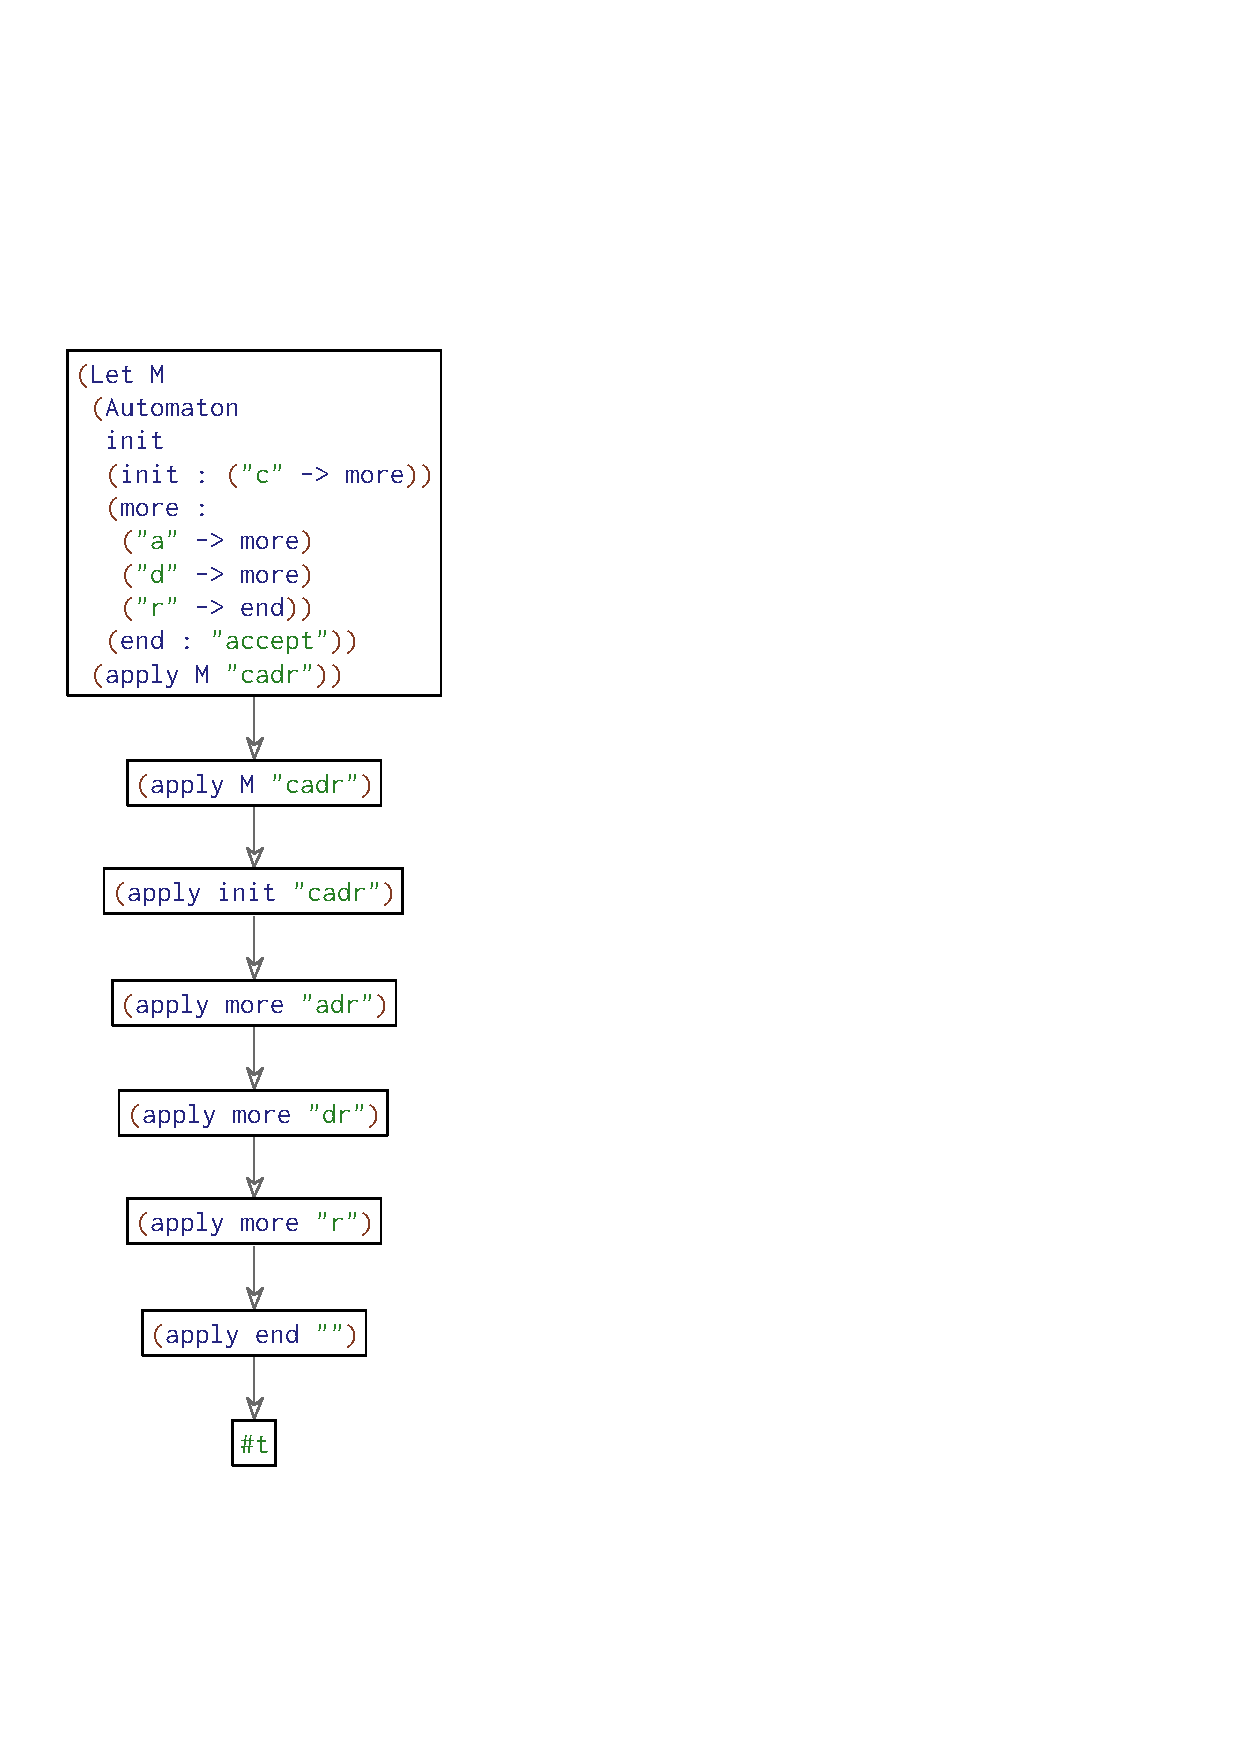
\includegraphics[width=0.45\columnwidth]{img/automaton-example}\hfill\mbox{}
\caption{Automaton macro execution example}
\label{fig:reval-automaton}
\end{figure}


\subsection{Return}
  Having first-class access to the current continuation is a powerful
  mechanism for defining new control flow constructs. Racket does so with
  the built-in function \Code{call/cc}, that takes a function of one
  argument and calls it with the program's current continuation. Using it,
  we can define a \Code{return} sugar that returns early from a function:
  \begin{Codes}
  Return(x) ->
    Let([Bind("\%RES", x)],
        [Apply(Id("\%RET"), [Id("\%RES")])]);

  Function(args, body) ->
    Lambda(args, Apply(Id("call/cc"),
                       [Lambda(["\%RET"], body)]));
  \end{Codes}
  (The definition of \Code{function} is necessary to mark the point that
  \Code{return} should return to.) With this definition in place, we can
  see evaluation sequences such as:
  \begin{Codes}
    (+ 1 ((function (x) (+ 1 (return (+ x 2)))) (+ 3 4)))
\SurfStep (+ 1 ((function (x) (+ 1 (return (+ x 2)))) 7))
\SurfStep (+ 1 (+ 1 (return (+ 7 2))))
\SurfStep (+ 1 (+ 1 (return 9)))
\SurfStep (+ 1 9)
\SurfStep 10
  \end{Codes}
  This example illustrates that our approach is robust enough to work even
  in the presence of dynamic control flow.


\subsection{Pyret: A Case Study}
\label{sec:reval-pyret}

Pyret, shown in \cref{sec:reval-pyret-example}, is a new language. It makes
heavy use of syntactic sugar to emulate the syntax of other programming
languages like Python. This sugar was implemented by people other than
this paper's authors, and written as a manual compiler, not as a set
of rules; it was also implemented without any attention paid to the
limitations of this work. Thus, the language makes for a good case
study for the expressiveness of our work.

We restricted our attention to sugar relevant to evaluation. Pyret has
builtin syntactic forms for writing tests, and can run code both in a
``check'' mode that only runs these tests, or in ``normal'' mode that runs
code. We focused on ``normal'' mode since it is most
relevant to evaluation. There were two pieces of sugar we
were unable to express and one that
required modification to show ideal surface steps; we
describe these in more detail below. 
As \cref{fig:reval-pyretsugar} shows, we were able to handle almost all
of Pyret's sugar. An example of the result in action was shown in
\cref{sec:reval-pyret-example}.

\begin{figure}
\begin{center}\small
\begin{tabular}{l | l c}
  \emph{\Sc{ast} Node} & \emph{Description} & \emph{Implemented?} \\ \hline
  fun & function declaration & yes \\
  when & one-arm conditional & yes \\
  if & multi-arm conditional & yes \\
  cases & multi-arm conditional & yes \\
  cases-else & multi-arm conditional & yes \\
  for & generalized looping construct & yes \\
  op & binary operators & yes \\
  not & negation & yes \\
  paren & grouping construct & yes \\
  left-app & infix notation & yes \\
  list & list expressions & yes \\
  dot & indirect field lookup & yes \\
  colon & direct field lookup & yes \\
  (currying syntax) & allowed in \Code{fun} and \Code{op} & yes \\
\hline
  graph & create cyclic data & no \\
  datatype & datatype declarations & no
\end{tabular}
\end{center}
\caption{Syntactic sugar in normal-mode Pyret}
\label{fig:reval-pyretsugar}
\end{figure}

We were unable to fully handle algebraic datatype declarations
because they splice one block of code into another in a non-compositional
manner; we believe these could be expressed by adding a block
construct that does not introduce a new scope (akin to Scheme's
\Code{begin}).

We were also unable to handle \Code{graph}, which constructs cyclic data.
It has a
complex desugaring that involves creating and updating placeholder values
and compile-time substitution. This could be solved either by expanding
the expressiveness of our system or by adding a new core construct to the
language. There is always a trade-off between the complexity of the core
language and the complexity of the desugaring; when a feature can only be
implemented through a highly non-compositional sugar like this, it may
make sense to instead add the feature to the core language.

Finally, the desugaring for binary operators needed to be modified to show helpful
surface evaluation sequences. The desugaring follows
a strategy similar to that of Python, by applying the \Code{\_plus} method
of the left subexpression to the right subexpression (the \Code{s} terms
are source locations, used for error-reporting):
\begin{Codes}
  Op(s, "+", x, y)  ->
    App(s, Bracket(s, x, Str(s, "_plus")), [y]);
\end{Codes}
Given the term \Code{1 + (2 + 3)}, we would expect evaluation to step
first to \Code{1 + 5} and then to \Code{6}. Unfortunately, {\Resugarer}
shows only this surface evaluation sequence:
\begin{Codes}
    1 + (2 + 3) \SurfStep 6
\end{Codes}
The core evaluation sequence reveals why:
\begin{Codes}
    1.["_plus"](2.["_plus"](3))
\CoreStep <func>(2.["_plus"](3))
\CoreStep <func>(<func>(3))
\CoreStep <func>(5)
\CoreStep 6
\end{Codes}
(\Code{<func>} denotes a resolved functional). To show the
term \Code{1 + 5}, Emulation requires that it desugar
precisely into one of the terms in the core sequence; but it desugars
to \Code{1.["\_plus"](5)}, which has a different shape than any of the
core terms.

The fundamental problem is the order of evaluation induced by this
desugaring: first the left subexpression is evaluated, then the
\Code{\_plus} field is resolved, then the right subexpression is
evaluated, then the ``addition'' is performed. We can obtain a more
helpful surface sequence by instead choosing a desugaring
that forces the left and right subexpressions to be evaluated fully before
resolving the operation, as shown in \cref{fig:reval-alt-plus}.

\begin{figure}[t]
\begin{Codes}
  Op(s, "+", x, y) ->
    Block(s,
    [ Let(s, Bind(s, "temp", ABlank),
             Obj(s, [Field(s, Str(s, "left"), x),
                     Field(s, Str(s, "right"), y)]))
    , App(s, Bracket(s, Bracket(s, Id(s, "temp"),
                                   Str(s, "left")),
                        Str(s, "_plus")),
             [Bracket(s, Id(s, "temp"),
                         Str(s, "right"))])]);
\end{Codes}
\caption{Alternate desugaring of addition}
\label{fig:reval-alt-plus}
\end{figure}
This desugaring constructs a temporary object \Code{\{left: x, right:
  y\}}, and then computes \Code{temp.left.\_plus(temp.right)}. Notice that
this desugaring \emph{slightly} changes the semantics of binary operators;
the difference may be seen when the right subexpression mutates the
\Code{\_plus} field of the left subexpression. In exchange, we obtain the
expected surface evaluation sequence:
\begin{Codes}
    1 + (2 + 3) \SurfStep 1 + 5 \SurfStep 6
\end{Codes}





\section{Related Work}

There is a long history of trying relate compiled code back to its
source. This problem is especially pronounced in debuggers for
optimizing compilers, where the structure of the source can be altered
significantly~\cite{hennessy-debugging}. Most of this literature
is based on black-box
transformations, unlike ours, which we assume we have full control
over.  As a result, this work tends to be very different in flavor
from ours: some of it is focused on providing high-level
representations of data on the heap, which is a strict subproblem of
ours, or of correlating back to source expression \emph{locations}, which
again is weaker than \emph{reconstructing a source term}.
For this reason,
this work is usually also not accompanied by strong semantic
guarantees or proofs of them.

One line of work in this direction is SELF's debugging
system~\cite{self-debugging}. Its compiler provides its debugger with
debugging information at selected breakpoints by (in part) limiting the
optimizations that are performed around them. This is a sensible approach
when the code transformation in question is optimization and can be turned
off, but does not make sense when the transformation is a desugaring
which is necessary to give the program meaning.

Another line of work in this direction is the compile-time macro error
reporting developed by Culpepper, et al.~\cite{fortifying-macros}.
Constructing useful error messages is a difficult task that we have not
yet addressed. It has a different flavor than the problem we address,
though: akin to previous work in debugging, any source terms mentioned in
an error appear directly in the source, rather than having to be
reconstructed.

Deursen, et al.~\cite{deursen:origin-tracking} formalize the concept of
tracking the origins
of terms within term rewriting systems (which in their case represent
the \emph{evaluator}, not the \emph{syntactic sugar} as in our
case). They go on to show various applications, including
visualizing program execution, implementing debugger breakpoints,
and locating the sources of errors.
Their work does not involve the use of syntactic sugar,
however, while our work hinges on the interplay between syntactic
sugar and evaluation. Nevertheless, we
have adopted their notion of origin tracking for our transformations.

Krishnamurthi, et al.~\cite{sk:mcmicmac} develop a macro system meant
to support a variety of tools, such as type-checkers and
debuggers. Tools can provide feedback to users in terms of the
programmer's source using source locations recorded during
transformation. The system does not, however, reconstruct source
terms; it merely point out relevant parts of the original source.  The
source tracking mechanisms are based on Dybvig, et al.'s macro
system~\cite{expansion-passing-style}.

Clements~\cite[page 53]{clements:thesis} implements an algebraic
stepper (similar to ours) for Racket---a language that has
macros---and thus faces precisely the same problem we address in this
paper. That work, however, side-steps these issues by handling a
certain fixed set of macros specially (those in the ``Beginner
Student'' language) and otherwise showing only expanded code.
On the other hand, it proves that its method of instrumenting a program to
show evaluation steps is correct (i.e., the instrumented program shows the
same evaluation steps that the original program produces),
while we only show that the lifted evaluation sequence is correct
with respect to the core stepper. Thus its approach could be
usefully composed with ours to achieve stronger guarantees.

Fisher and Shivers~\cite{ziggurat} develop a framework
for defining static semantics that connect the
surface and core languages. They show how to effectively \emph{lower}
a \emph{static} semantics from a surface language to its core
language. This is complementary to our work, which
shows how to \emph{lift} a \emph{dynamic} semantics from core to surface.
This exposes a fundamental difference in starting assumptions:
they assume the surface language has a static semantics, while we assume
its semantics is \emph{defined} by desugaring.

In a similiar vein, Lorenzen and Erdweg \cite{typechecking-exts} give a
method for ensuring the type soundness of syntactic extensions by lowering
author-provided typing rules for the surface language onto the core
language's type system (and automatically verifying that soundness is
entailed). Thus their work does for type checking what ours does for
evaluation: it provides a surface type checker guaranteed to be sound with
respect to the core language, while ours produces a surface evaluator
guaranteed to emulate the core language.

Model-driven software engineering also draws heavily on
bidirectional transformation, because systems are expected to be written
in a collection of domain-specific languages that are transformed into
implementations. These uses tend to be \emph{static}, rather
than addressing the inverse-mapping problem in the context of system
execution (see the survey by
Stevens~\cite{bidirectional-model-transfs}).
When the problem we address does arise in this area, it is typically the
case that either (i) both the source and target models have
implementations, so that surface-level execution traces can be obtained
by evaluating in the surface language directly~\cite{Perera-slicing}, or
(ii) the surface information sought is more limited than the reduction
sequence we provide (in the same ways as for debuggers for optimizing
compilers, as described earlier).
Applying our results to this area is future work.
